


\chapter{Экспериментальная часть}\label{exp}
%\addcontentsline{toc}{chapter}{4 Экспериментальная часть}

Оценка качества работы алгоритмов. Экспериментальное сравнение работы различных алгоритмов нахождения среднего арифметического матрицы
(зависимость времени выполнения от размерности матриц).

\section{Технические характеристики}\label{texcharacters}

Технические характеристики устройства, на котором выполнялось тестирование:

\begin{enumerate}
    \item процессор: Intel® Core™ i3-7100U CPU @ 2.40GHz × 4; 
    \item память: 11,6 GiB;
    \item операционная система: Ubuntu 20.04.1 LTS.
\end{enumerate}

\section{Примеры работы}\label{examples}

На рисунке \ref{ris:w1} показан пример работы.

%\begin{figure}[H]
%    \center{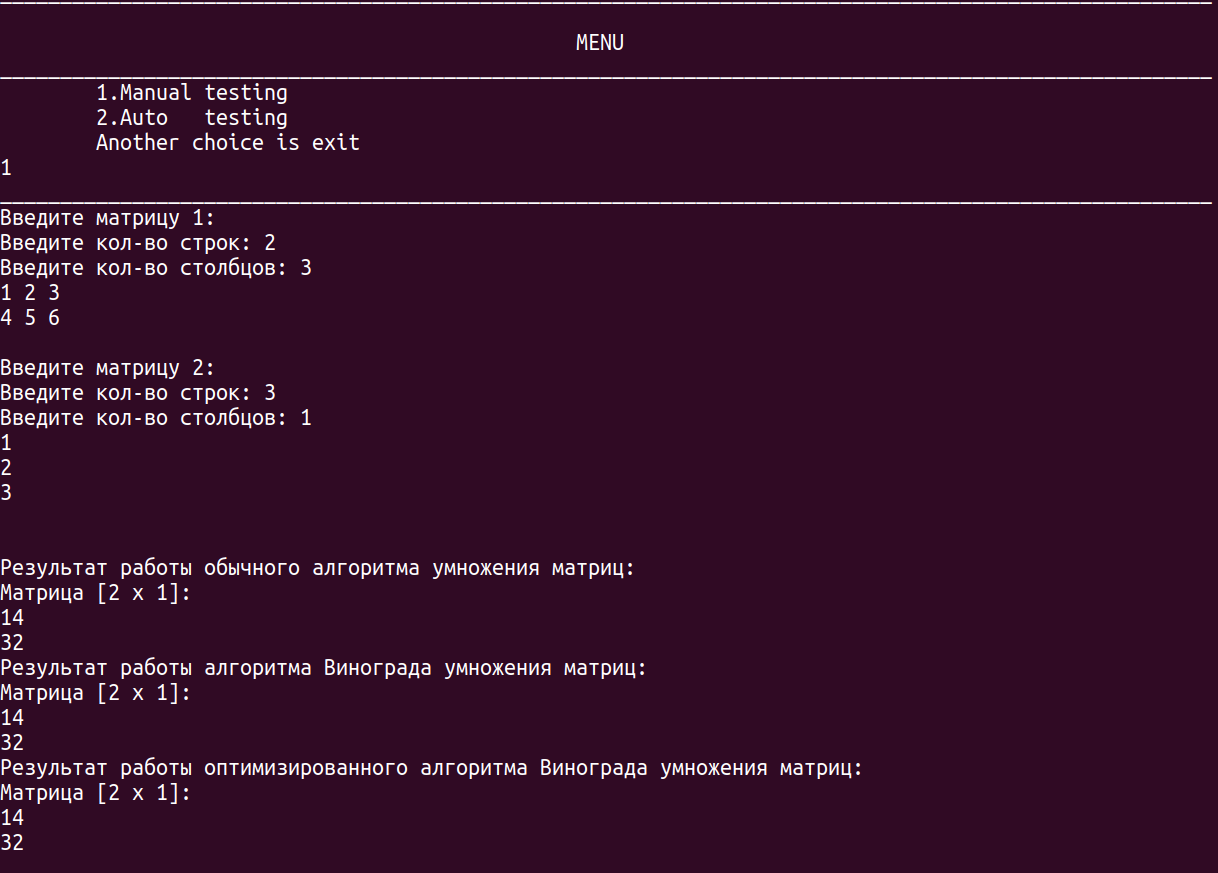
\includegraphics[scale=0.35]{w3}}
%    \caption{Ручное тестирование: тест 3}
%    \label{ris:w4}
%\end{figure}
  
\begin{figure}[H]
    \center{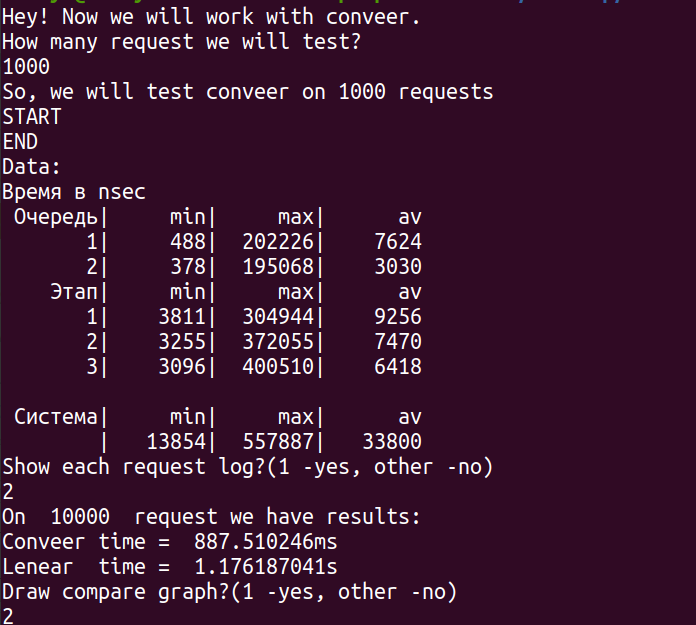
\includegraphics[scale=0.25]{w1}}
    \caption{Пример работы 1}
    \label{ris:w1}
\end{figure}

\section{Замеры времени}\label{experimentgraph}

Так как поиск в словаре считается короткой задачей, воспользуемся
усреднением массового эксперимента. Для этого сложим результат работы
алгоритма n раз (n >= 10), после чего поделим на n. Тем самым получим
достаточно точные характеристики времени. Сравнение произведем при n =
10000



Таблица \ref{tab:resulttime} содержит результаты замеров времени.
 Используются следующие обозначения all\_search - алгоритм полного перебора,
 bin\_search - алгоритм бинарного поиска, seg\_search-алгоритм поиска по сегментам.


\begin{table}[ht]
    \caption{Замеры времени (в нсек)}
    \centering
    %\scriptsize
\begin{tabular}{ l | l | l | l | l | }  
    Название функции&         ключ&         Время&          Результат\\\hline\hline

    all\_search&            0&               2.280110&         NONE\\ 
    all\_search&  23400005678&             0.931010&Kathleen Johnson\\
    all\_search&  23401515678&              1.000850& Donna Weaver\\
    all\_search&  23420735678&              2.123130&Kenneth Hunter\\\hline
    
    bin\_search&            0&               0.984990&         NONE\\
    bin\_search&  23400005678&            0.961090&Kathleen Johnson\\
    bin\_search&  23401515678&           0.977360& Donna Weaver\\
    bin\_search&  23420735678&            0.961380&Kenneth Hunter\\\hline
    SEGMENTS COUNT =  1\\
    seg\_search&            0&             0.974430&         NONE\\
    seg\_search&  23400005678&            0.947140&Kathleen Johnson\\
    seg\_search&  23401515678&             0.948310& Donna Weaver\\
    seg\_search&  23420735678&          0.958050&Kenneth Hunter\\\hline
    SEGMENTS COUNT =  51\\
    seg\_search&            0&            0.958450&         NONE\\
    seg\_search&  23400005678&             0.958310&Kathleen Johnson\\
    seg\_search&  23401515678&           0.957090& Donna Weaver\\
    seg\_search&  23420735678&          0.959080&Kenneth Hunter\\ \hline
 
\end{tabular}
\label{tab:resulttime}
\end{table}



%На рисунках \ref{ris:graph1} и \ref{ris:graph2} показаны графические результаты сравнения исследуемых алгоритмов по времени. 

%\begin{figure}[H]
 %   \center{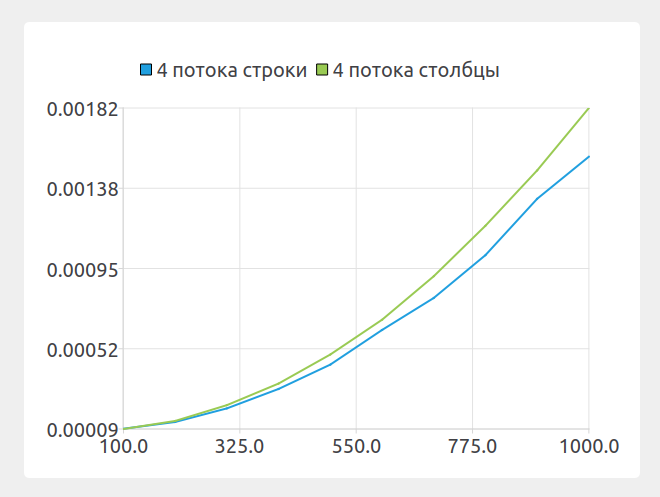
\includegraphics[scale=0.45]{graph3}}
  %  \caption{Сравнение распараллеленого по строкам и столбцам алгоритмов (при 4 потоках)}
   % \label{ris:graph2}
%\end{figure}

%\begin{figure}[H]
  %  \center{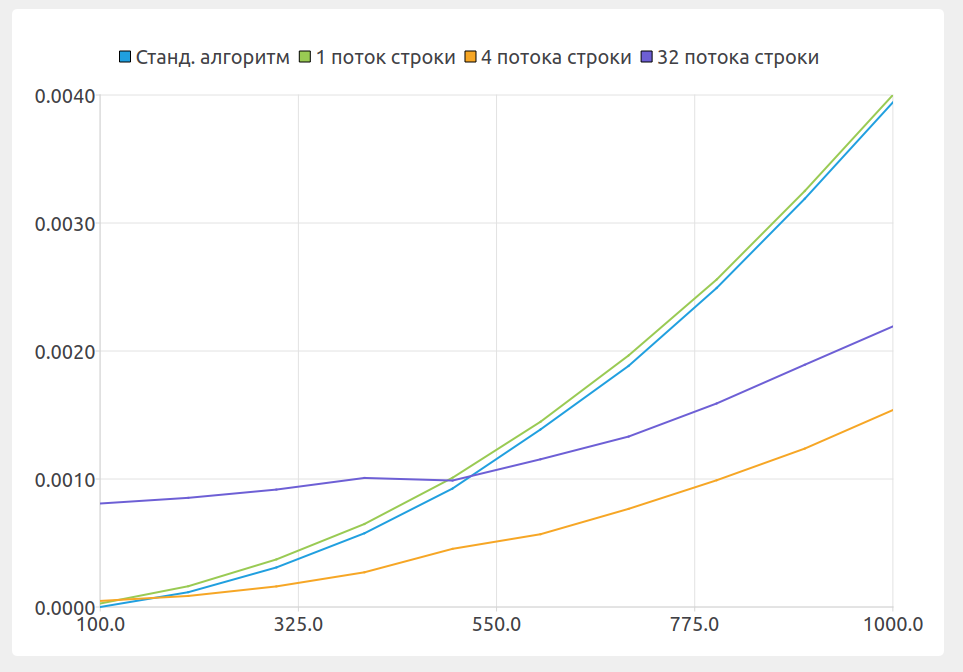
\includegraphics[scale=0.4]{graph5}}
 %   \caption{Сравнение алгоритмов стандартного, распараллеленого по строкам на 1, 2, 4, 32 потока}
   % \label{ris:graph1}
%\end{figure}

\section{Сравнительный анализ алгоритмов}\label{comparepart}

По результатам экспериментов можно заключить следующее:
\begin{enumerate}
    \item представлен результат поиска первого значения. Выигрыш алгоритма
    поиска полным перебором обосновывается тем, что он тратит лишь одно сравнение для того, чтобы найти первый ключ, в том время, когда
    бинарный поиск затрачивает гораздо больше сравнений. Частичный анализ работает чуть медленнее, так как ему нужно произвести дополни-
    тельное сравнение первых букв;
    \item представлен результат поиска среднего значения: выигрыш бинарного поиска в том что он находит середину за одну итерацию; 
    \item представлен результат поиска произвольного ключа: алгоритм полного перебора работает медленнее всех;
    \item произведено аналогичное сравнение, только в качестве искомого ключа взят несуществующий. 
    Аналогично поиск полным перебором затрачивает больше всего времени по вышеописанной причине.
\end{enumerate}

\section{Вывод экспериментальной части}\label{experimentresult}

В данном разделе было произведено сравнение трех алгоритмов. По
результатам исследования было доказано, что алгоритм полного перебора в
основном работает медленнее всех, за исключением, когда ключ лежит достаточно близко к началу

\addcontentsline{toc}{chapter}{{Заключение}}
\chapter*{Заключение}\label{exit}

В данной работе были изучены алгоритмы поиска по словарю. 
Получены практические навыки реализации приведенных алгоритмов. 
Проведён сравнительный анализ алгоритмов по времени. 
Экспериментально подтверждены различия в эффективности алгоритмов с указанием лучших и худших случаев. 
Цель работы достигнута, решены поставленные задачи. 
